\documentclass[Bachelorarbeit.tex]{subfiles}
\begin{document}
\chapter{Konzeption}
\label{chap:entwicklung}

\section{Konzept}
\label{chap:entwicklung:sec:konzept}

\ideas{Konzept für die ersten Entwürfe aus den Ergebnisse der Analyse mergen}

\section{Interviews}
\label{chap:analyse:sec:interviews}
Dieser Teil beschäftigt sich mit der Fragestellung, wie Personen ihre Außendienstlichen Tätigkeiten organisieren, welchen Herausforderungen sie im beruflichen Alltag gegenüberstehen und welche Verbesserungen sie sich wünschen. 
Für diesen Zweck sollen Interviews und Hand-ons  geführt werden, die sich an einem Leitfaden orientieren (siehe Anhang: \nameref{anhang:leitfaden_interviews}). 
Das Ziel dieser Interviews besteht darin, ein besseres Gefühl für den Ist-Zustand zu bekommen und Anhand dieser Erkenntnisse die möglichen Defizite zu analysieren.
Des weiteren bietet der Ansatz die Möglichkeit, Verbesserungswünsche und Ideen von Personen aus d1er Domäne zu erhalten ohne das sie zuvor durch den Blick aus technischer Sicht verfälscht wurden.

\section{Ergebnisse der Interviews}
Es wurden drei Interviews mit Personen aus verschiedenen Bereichen durchgeführt. 
Wie zu erwarten war, gibt es zwar grundlegende Ähnlichkeiten der Workflow, allerdings unterscheiden sie sich in der Ausprägungen.\\
\\
Für eine bessere Übersicht, sind die Erkenntnisse aus denn Interviews in die drei Kategorien: \nameref{subsubsec:Ergebnisse der Interviews:gemeinsamkeiten}, \nameref{subsubsec:Ergebnisse der Interviews:probleme} und \nameref{subsubsec:Ergebnisse der Interviews:ideen} zusammengefasst und werden jeweils separat betrachtet.

\subsection*{Gemeinsamkeiten}
\label{subsubsec:Ergebnisse der Interviews:gemeinsamkeiten}
Abstrakt gesprochen, unterscheiden sich die Workflows in ihren Grundzügen nicht deutlich von einander (siehe abb.: \ref{fig:abstrakterWorkflowPlannung} - \nameref{fig:abstrakterWorkflowPlannung}). 
Es besteht eine Grundmenge von Möglichkeiten (beispielsweise Kunden\_innen oder Stammdaten). 
Aus dieser Grundmenge wird, mit Hilfe von Filterungs- und/oder Anreicherungsschritten, die Teilmenge der relevanten Möglichkeiten gebildet, was wiederum beliebig oft wiederholt wird (für jedes Entscheidungskriterium).
Nachdem die Teilmenge der relevanten Möglichkeiten, den Anforderungen des Szenarios entspricht, wird mit der Auswahl der Elemente fortgefahren.
Die Menge dieser Elemente bilden schlussendlich die getroffene Auswahl für die Planung.\\
\\
Bei diese Schilderung handelt es sich allerdings nur um den kleinsten gemeinsamen Nenner der geführten Interviews.
Die Unterschiede liegen dabei in den Details, wie beispielsweise die Auswahl für die Teilmenge der relevanten Möglichkeiten gebildet wird.
Speziell die Probleme, die in den jeweiligen Details auftreten werden im folgenden Abschnitt genauer erläutert.

\begin{figure}[h]
	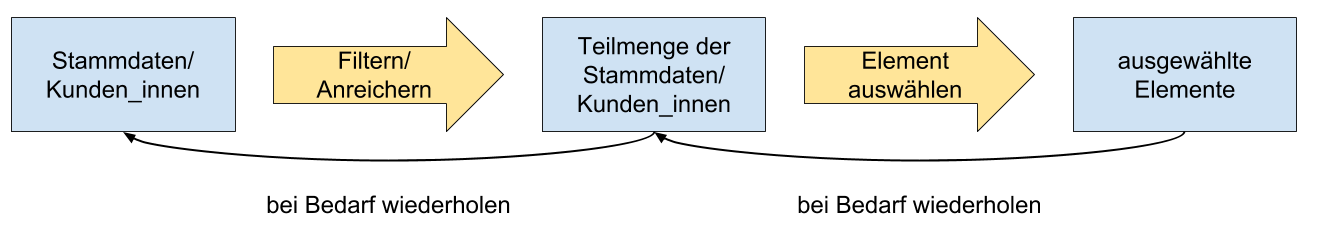
\includegraphics[width=\linewidth]{img/analyse/abstrakterWorkflowPlannung}
	\caption[abstrakter Plannungsworkflow]{lang}
	\label{fig:abstrakterWorkflowPlannung}
\end{figure}

Mithilfe der Interviews, wurden zwei weitere Phasen identifiziert, welche für die Praxis von hoher Relevanz sind und im vorhergehenden Kapitel noch nicht beachtet wurden.
Dabei handelt es sich zum einen um die Unterstützung während der Durchführung der Außendiensttätigkeit und zum anderen um die Aufbereitung der Daten nach der Außendiensttätigkeit.

\subsection*{Probleme}
\label{subsubsec:Ergebnisse der Interviews:probleme}
Alle in den \nameref{chap:analyse:sec:interviews} besprochenen Workflows haben an gewissen Stellen ihre Schwachpunkte. 
Das Ziel dieses Abschnitts besteht darin, die Probleme zusammen zu fassen und somit eine Übersicht zu gestalten, die als Grundlage für die \nameref{chap:entwicklung} des Prototypen dient. 
in folgender Übersicht (siehe Tabelle: \ref{tab:problemeInterviews} - \nameref{tab:problemeInterviews}) wird, anhand von acht Punkten, aufgezeigt welche Engpässe, in welchen Interview festgestellt wurde.

\def\arraystretch{1.5} %  1 is the default, change whatever you need
\begin{table}[h]
	\begin{tabular}{|p{5cm}|p{2,25cm}|p{2,25cm}|p{2,25cm}|}
		\hline  
		& \ctab \nameref{anhang:interview1} 
		& \ctab \nameref{anhang:interview2} 
		& \ctab \nameref{anhang:interview3} \\ 
		\hline 
		\nameref{p1}
		& \ctab X
		& \ctab X
		& \ctab  \\ 
		\hline 
		\nameref{p2}
		& \ctab  X
		& \ctab X
		& \ctab  \\ 
		
		\hline 
		\nameref{p3}
		& \ctab  
		& \ctab X
		& \ctab X \\ 
		\hline 
		\nameref{p4}
		& \ctab 
		& \ctab  X
		& \ctab X \\ 
		\hline 
		\nameref{p5}
		& \ctab 
		& \ctab (indirekt)
		& \ctab X \\ 
		\hline 
		\nameref{p6}
		& \ctab X
		& \ctab X
		& \ctab  \\ 
		\hline 
		\nameref{p7}
		& \ctab 
		& \ctab X
		& \ctab X \\
		\hline 
		\nameref{p8}
		& \ctab
		& \ctab X
		& \ctab X \\
		\hline 
	\end{tabular} 
	\caption[Zusammenfassung der Probleme]{Übersicht über die zusammengefassten Probleme der einzelnen Interviews}
	\label{tab:problemeInterviews}
\end{table}

\subsection*{Zusammengefasste Probleme}
\ideas{Eventuell die Punkte weiter zusammenfassen?}

\paragraph*{1. Daten sind auf verschiedene Medien und Systeme verteilt}
\label{p1}
Bei zwei der durchgeführten Interviews ist aufgefallen, das die benötigten Daten für die Planung auf unterschiedliche Systeme verteilt sind.
Dies geht soweit, das sogar Medienbrüche (Papierkalender - siehe: \nameref{anhang:interview1}) stattfinden.
Bei dem Beispiel, handelt es sich um wiederkehrende Termine, die leicht im Kalender übersehen werden können. Durch solch ein versäumen, entsteht ein Umplanungsverfahren, welches Zeit- und Ressourcen aufwendiges ist.\\
\\
Im Gespräch stellt sich heraus, dass es für diese Patchwork-Konstruktion zwei Ursachen gibt.
Diese liegen zum einen darin, dass den Anwender\_innen nicht der gesamte Funktionsumfang ihrer Lösung bekannt ist, sowie aus Gewohnheit und/oder persönlicher Vorliebe andere Werkzeuge präferiert werden.
Zum anderen, stellen die vorhandenen Organisationswerkzeuge nicht denn benötigten Funktionsumfang zur Verfügung, woraufhin dritte Systeme oder Medien als Unterstützung evaluiert und eingesetzt werden. 

\paragraph*{2. Filterung von Kunden auf Basis von geografischen Grenzen (Stadt, Land, etc.)}
\label{p2}
\ideas{
	\begin{itemize}
		\item Persönliche Ortskenntnisse notwendig
		\item - Probleme bei Vertretungen von anderen Einzugsgebieten
		\item Filterung auf Basis von PLZ
		\item Zwei Kunden können nebeneinander liegen (aneinander liegenden Stadträndern), werden aber auf Grund von harten Grenzen ausgefiltert.
	\end{itemize}
}

\paragraph*{3. Umständliche/mehrfache Filterungsschritte}
\label{p3}
\ideas{
	\begin{itemize}
		\item Teilweise müssen erst Zwischenabfragen getätigt werden und die Ergebnisse notiert werden um sie anschließend im nächsten Filter wieder einzutragen - Filterworkflow 
		\item Teilweise Filtern über verschiedene Systeme/Software hinweg mit Copy and Paste
	\end{itemize}
}

\paragraph*{4. Keine Möglichkeit Routen zu verwalten }
\label{p4}
\ideas{
	\begin{itemize}
		\item wiederholende Routen mit minimalen oder keinen geänderten Parametern
		\item ausgewählte Kunden werden auf PostIts übertragen (Interview II) - Aufwendig und Fehleranfällig
	\end{itemize}
}

\paragraph*{5. Fehlende Visualisierung von Distanzen}
\label{p5}


\paragraph*{6. Fehlende Überblick welcher Kunde ist in der Nähe ist}
\label{p6}
\ideas{
	\begin{itemize}
		\item Speziell bei spontanen Änderungen im Außendienst, Termin verschiebt sich oder fällt aus.
	\end{itemize}
}

\paragraph*{7. Fehlende Möglichkeiten für kundenspezifischen Metadaten}
\label{p7}
\ideas{
	\begin{itemize}
		\item Laut allen drei Interview sind Hinterlegungen für interne Anmerkungen über Kunden bzw. Ansprechperson sehr essentiell und auch in der Planung berücksichtigt
		\item Werden oft nur als Notizfelder von Programmen angeboten.
		\item Evtl. nicht relevant bzw. als zusätzliche Information 
	\end{itemize}
}

\paragraph*{8. Umständliche Exportmöglichkeiten von Kunden-/Stammdaten}
\label{p8}
\ideas{
	\begin{itemize}
		\item Stammdatenblätter sind für die Durchführung wichtig
		\item Werden vor der Tour händisch exportiert und ausgedruckt
	\end{itemize}
}


\subsection*{Wünsche/Ideen}
\label{subsubsec:Ergebnisse der Interviews:ideen}

Für die Analyse, an dieser Stelle, sind zwei wichtige Kategorien.  



\subsection{Persona}
\label{persona}
\ideas{Entwicklung der Persona beschreiben, evtl noch in die Analyse packen}

\section{Design-Entwurf}
\label{chap:entwicklung:sec:design_entwurf}

merken der Kartenposition

\ideas{Dokumentation des Entwicklungsprozesse vom \nameref{chap:entwicklung:sec:konzept} zum \nameref{chap:entwicklung:sec:design_entwurf:sub:mockUps} \\
	\\
	Entwicklung nach "'user centered design"
	\\
	UI-Design Studie: 
	\begin{itemize}
		\item Welche Darstellung unterstützt den/die Anwender\_in am ehesten
		\item Map- vs. List-View (evtl. weitere Darstellungsmöglichkeiten)
		\item Sinnvolle Visualisierung von Prioritäten 
		\item Auswahl basierte Darstellung für UI 
	\end{itemize}}

\subsection{Ziele der Gestaltung}
\label{chap:entwicklung:sec:design_entwurf:subs:ziele_der_gestaltung}

\ideas{Definition auf welche Ziele hingearbeitet werden soll - Einfluss der Erkenntnisse aus Abschnitt: \nameref{chap:entwicklung:sec:konzept}}

\begin{comment}
Um die Ziele der Gestaltung definieren zu können muss zuerst analysiert werden, wie die Zielgruppe ihre Wünsche und Erwartungen an die Applikation definiert.\\

\subsubsection*{Ziel: Übersichtlichkeit}
\label{subsub:ziel_uebersichtlichkeit}
Eine klare und aufgeräumte Oberfläche ist notwendig, um die Unterstützung der Benutzer zu maximieren. 
Dazu zählt das Aufteilen der Inhalte in sinnvolle und logische Gruppen unter der Berücksichtigung der Arbeitsabläufe.


\subsubsection*{Ziel: Vertraute Umgebung}
\label{subsub:ziel_vertraute_umgebung}
Durch das Erzeugen einer vertrauten Umgebung sollen die Nutzer bekannte Elemente ihrer Plattform in der Applikation wiedererkennen.
Dadurch sollen die Einarbeitungszeiten in die Applikation minimiert, sowie der Wiedererkennungswert von plattformtypischen Elementen wie beispielsweise die Navigation durch das Programm, maximiert werden.
Es wird versucht, dass die Benutzer jeder Zeit das Gefühl haben, dass sie das Programm vollständig kontrollieren.
Dadurch soll den Nutzern die Angst genommen werden "`etwas falsches zu machen"'.
Für die Realisierung dieses Zieles muss sich die Applikation an dem Standartverhalten der jeweiligen Plattform orientieren.
\newpage
\end{comment}


\subsection{Mock-Ups - Prototyp Entwicklung}
\label{chap:entwicklung:sec:design_entwurf:sub:mockUps}

\ideas{Dokumentation der Entstehung sowie Überlegungen des ersten Prototypen}

\begin{comment}
Um schon in einem frühen Stadium des Entwicklungsprozesses\\ Rückmeldungen über die Bedienbarkeit des Programmes zu erhalten, empfiehlt es sich, in die Entwicklung von Mock-ups zu investieren.
Unter Mock-Ups versteht man einen nicht funktionellen Prototypen. 
Dies bedeutet, dass der Prototyp nicht programmiert, sondern mit einem Bildbearbeitungsprogramm erzeugt wird.
Dabei wird für jede Ansicht ein eigener Prototyp "`gezeichnet"'. 
Anschließend werden mit Personen aus der Zielgruppe die einzelnen Szenarios der Applikation simuliert. 
Während des Testes sollen die NutzerInnen den Ablauf des Programmes, die erwarteten ihrer Ergebnis von Interaktionen sowie ihre Emotionen so detailliert wie möglich kommentieren.  
Mithilfe des Testes lässt sich feststellen, wie schlüssig die Arbeitsabläufe sind, ob die Funktionalität der Oberfläche verständlich ist und ob die Reaktionen des Programmes mit den Erwartungen der Benutzer übereinstimmen. 
Der Prozess des \texttt{Paper Prototyping} sollte nicht einmalig, sondern in Form eines iterativen Entwicklungsprozess durchgeführt werden. 
Dies bedeutet, dass auf der Basis der erhaltenen Rückmeldungen die Mock-Ups optimiert und die Test wiederholt werden.
Der Test kann als positiv betrachtet werden, wenn die Rückmeldungen der Probanden mit den zuvor definierten Design-Zielen (siehe Abschnitt: \nameref{sub:ziele_der_gestaltung}) übereinstimmen.\\
\\
Die Mock-Ups der Beispiel-Applikationen befinden sich im Anhang:  \nameref{chap:diagramme_und_bilder} unter dem Abschnitt: \nameref{sec:mock_ups}. 
\end{comment}

\newpage




\end{document}
